\section{Solver Convergence}
\subsubsection{NACA0012}
Figure \ref{fig:sc_NACA0012} shows the solver convergence for the NACA0012
testcase. The baseline implementation and the final state when writing this
report (modified) is shown. Both states were run once with 1 and 6 cpus.

\begin{figure}[H] \centering
    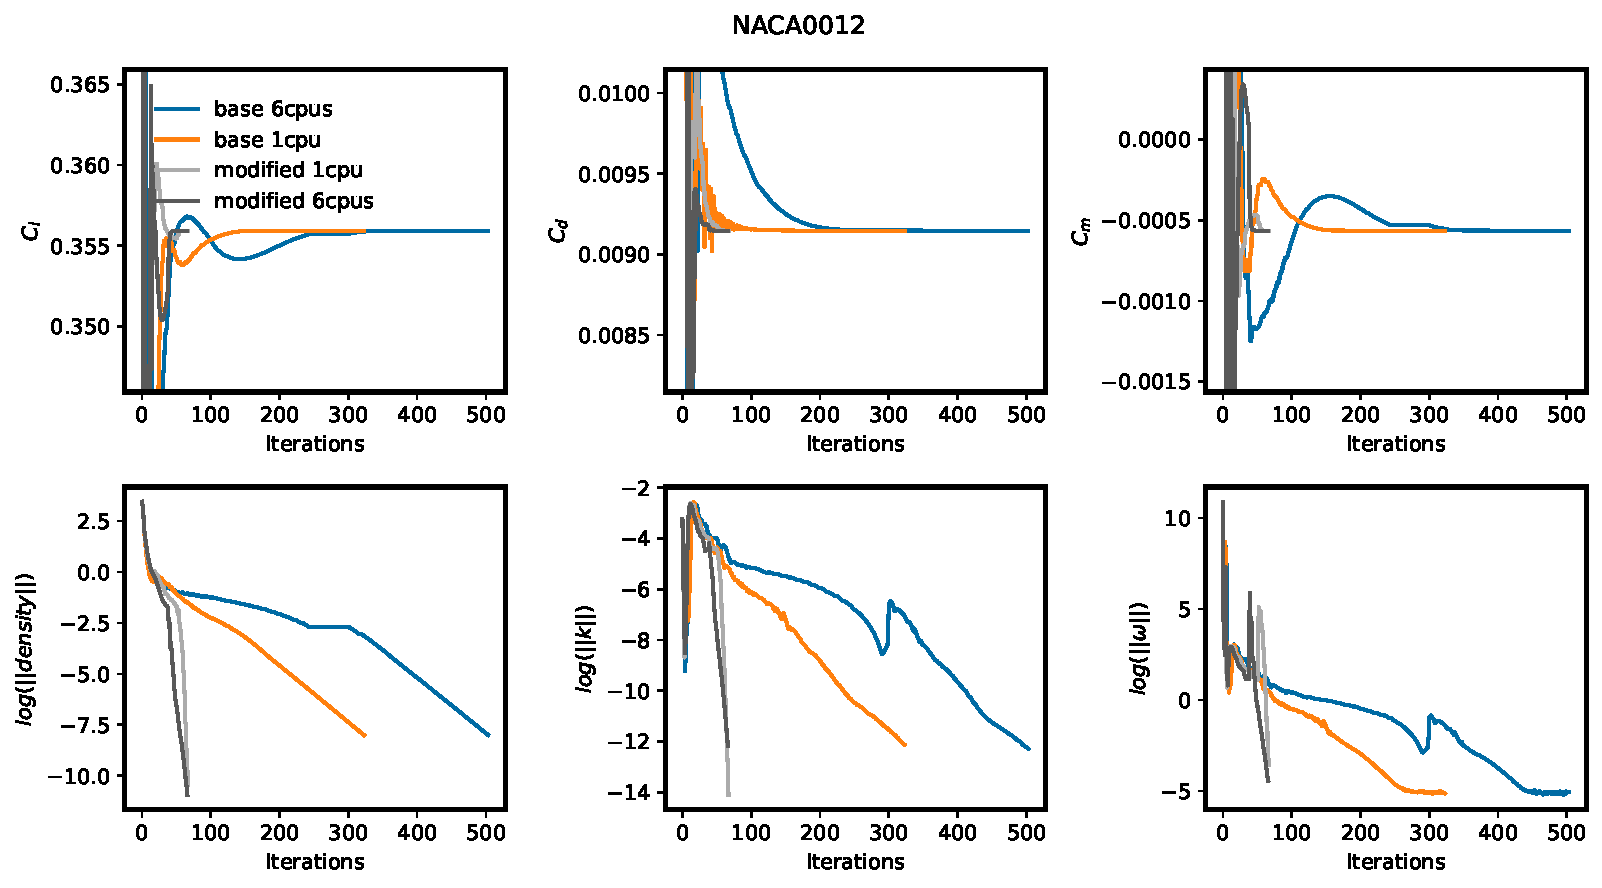
\includegraphics[width=1.0\textwidth]{plots/sc_NACA0012}
    \caption{Convergence history for NACA0012 testcase.}
    \label{fig:sc_NACA0012}
\end{figure}

\noindent Lets take a look at the baseline implementation first. It was
obtained using the ANK solver and a decoupled DADI solver for the turbulence
model. For the turbulence model, a total of 20 sub iterations were used. When
looking at the functions values (top row), it can be seen that 1 and 6 cpus
reach the same value. But 6 cpus need more iterations. It is not quite clear
what causes this, but it is a known phenomenon for low cpu counts and vanishes
when this number is increased. Production runs usually require tens or even
hundrets of cpus and thus this is not considered detrimental.


Now, lets look at the modified curves. Here, SST was differentiated and the
turbulence ANK and fully coupled CANK solvers are available. Annectdotal
evidence suggest SST is highly non-linear. This is especially true for the
inital stages of convergence. Due to this\footnote{The author believes the ANK
solver does some finite-differencing for some terms under the hood.}, the
turbulence DADI solver is way more efficient early on. Thus, at the beginning,
the regular ANK solver with decoupled DADI was used. But once a relative
convergence of 1e-6 is reached, the second order coupled ANK (CSANK) is
engaged. Once it gets traction, it exhibits almost Newton-like convergence. The
number of cpus does not really affect the number of iterations needed. It is
also obvious that the modified version approaches the same function values as
the baseline implementation. 




\subsubsection{RAE2822}
Figure \ref{fig:sc_RAE2822} shows a similar convergence plot for the RAE2822
testcase. Once again, the baseline and modified version with each 1 and 6 cpus
is plotted. It is important to note that this case is somewhat hard as it lies
in the transsonic regimes where shocks appear. But at the same time, it is even
coarser than the naca case which makes it hard to resolve them properly.

\begin{figure}[H] \centering
    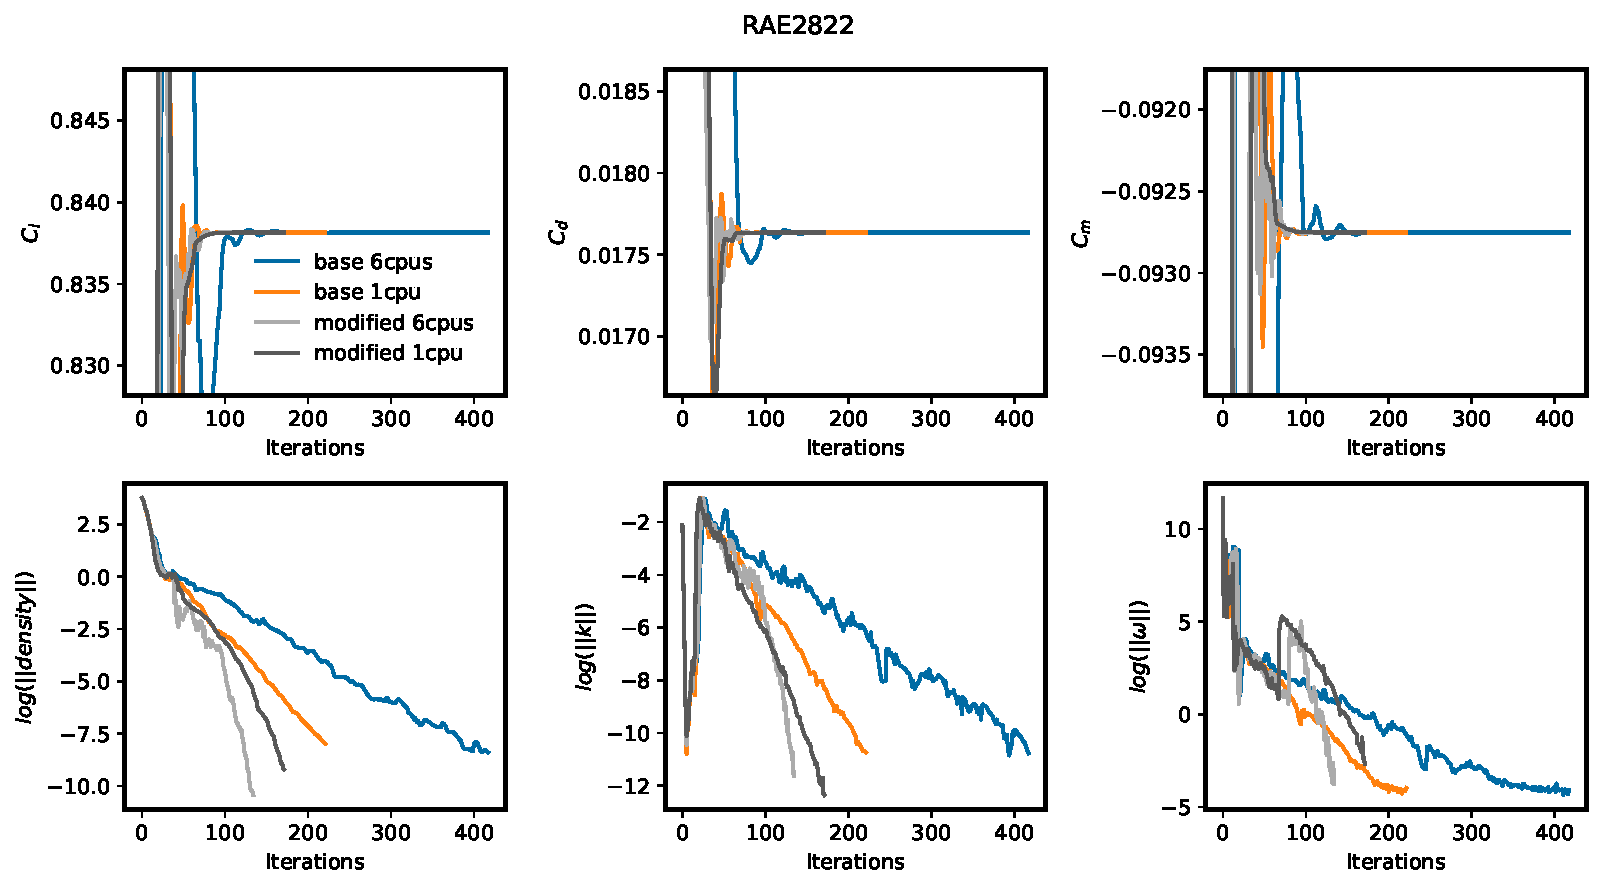
\includegraphics[width=1.0\textwidth]{plots/sc_RAE2822}
    \caption{Convergence history for RAE2822 testcase.}
    \label{fig:sc_RAE2822}
\end{figure}

\noindent First, lets glance ath the baseline. This has also been obtained
using the ANK solver for the flow variables and the DADI solver for the
decoupled turbulence variables. A similar pattern to the NACA
testcase appears: 1 cpu takes only half the iterations of what 6 cpus need.
But, the converged values are the same. When comparing the general line pattern
to the NACA testcase, it appears to be more 'wiggly' here. The author belieaves
this is due to the coarse mesh and transsonic regime. This probably increases
the sensitivity to the CFL number. During convergence, the ANK solver increases
the CFL number based on the current relative convergence. But the high
sensitivity makes the solver unstable and i starts to diverge. Once this is
detected, the CFL number is lowered again. This should be avoidable, but maybe
more tuning or even a change to the CFL-ramping algorithm is needed.

When looking at the modified version, a similar picture to NACA emerges. The
strategy was the same, first use ANK with DADI and once a relative convergence
of 1e-6 is reached, the CSANK solver is enganged which shows almost Newton-type
convergence. Although the contrast is not as big. But it also has to be noted
that that the before mentioned CFL dependence played a role here and some
parameters had to be clipped to increase robustness at the cost of convergence.



% FDPC


\section{SST testcases}

\section{Grid Convergence}

\section{Partial derivatives}

\section{Total derivatives}
